\documentclass{article}
\usepackage[utf8]{inputenc}   
\usepackage[french,english]{babel}
\usepackage[T1]{fontenc}

%%% Packages %%%

%Mise enpage
\usepackage{lmodern}
\usepackage{fullpage}

%Images et légendes
\usepackage{graphicx}
\usepackage{wrapfig}
\usepackage{caption}

%Autre
\usepackage{physics}
\usepackage{hyperref}


%Titre
\title{Équation d'état de Van der Waals et élément de matrice d'un 
opérateur hermitien}
\author{Nicolas Englebert}
\date{24 avril 2015}

\begin{document}

%\maketitle
\section{Équation d'état de Van der Waals}
\subsection{Courbe spinodale}
	\begin{wrapfigure}[13]{r}{2cm}
		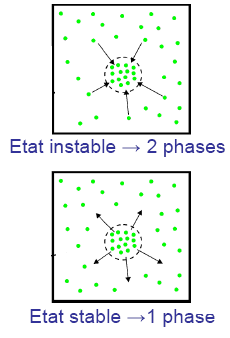
\includegraphics[scale=0.37]{images/image8.png}
		\captionof{figure}{ }
	\end{wrapfigure}
	Un gaz réel possède une transition liquide vapeur dont la pression est donnée par l'\textit{équation de Van der Waals}
	\begin{equation}
	p = \frac{RT}{v-b}-\frac{a}{v^2}
	\end{equation}
	
	En étudiant la variation de la pression par rapport au volume à température constante, deux cas sont possibles :
	\begin{equation}
	\left(\frac{\partial p}{\partial v}\right)_T\ est\ \ \left\{\begin{array}{l}
	< 0 : \text{stable }\rightarrow 1\ \text{phase}\\
	> 0 : \text{instable }\rightarrow 2\ \text{phases}
	\end{array}\right.
	\end{equation}
	\begin{wrapfigure}[14]{l}{5cm}
	\vspace{-5mm}
		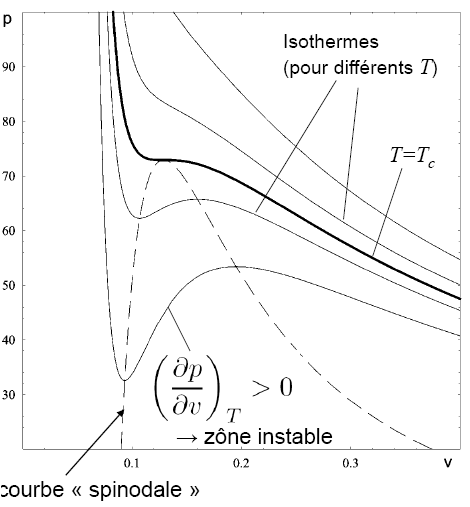
\includegraphics[scale=0.35]{images/image9.png}
		\captionof{figure}{Courbe spinodale}
	\end{wrapfigure}
	Si la dérivée est positive, c'est que l'on se trouve dans le cas spécial ou $P$ augmente avec $V$ (contre-intuitif) et que deux phases sont présentes. Si ce n'est pas le cas, on observe bien une diminution de la pression avec l'augmentation du volume (effet "normal", $PV$ = cste pour un gaz parfait).
	\\
	Égalons cette dérivée à zéro. On obtient dès lors : 
	\begin{equation}
	RT = 2av^{-3}(v-b)^2
	\end{equation}
	
	En isolant $RT$ dans l'expression de Van der Waals ci-dessus et en le remplaçant ici, on obtient :
	\begin{equation}
	p_{sp} = av^{-3}(v-2b)
	\end{equation}
	qui est la \textbf{courbe "spinodale"}, c'est à dire la courbe qui détermine les états instables\footnote{A l'intérieur de la courbe spinodale. A l'extérieur : stable.} qui mènent spontanément à la formation de deux phases : liq. et vap. Sous cette courbe, on voit que $P$ augmente avec $V$ (cf. plus haut).\\
	
	Une isotherme est définie par une température constante : deux points sur une isotherme ont donc la même température. Pour une même pression ($y = cste$) on se trouve à l'équilibre mécanique. L'équilibre chimique correspond à $\mu_A = \mu_B$.
	
	
\section{"Élément de matrice" d'un opérateur $\hat{A}$}
Soit
\begin{equation}
\ket{u} = \left(\begin{array}{c}
u_1\\
u_2\\
\vdots\\
u_n
\end{array}\right), \qquad \bra{v} = (v_1^*\ v_2^*\ \dots\ v_n^*), \qquad 
\hat{A}\ket{u} = \left(\begin{array}{ccc}
a_{11} & \dots & a_{1n}\\
\vdots &\ddots &\vdots\\
a_{n1} & \dots & a_{nn}
\end{array}\right)\left(\begin{array}{c}
u_1\\
u_2\\
\vdots\\
u_n
\end{array}\right)
\end{equation}
Nous avons alors
\begin{equation}
\bra{v}\left(\hat{A}\ket{u}\right) = \underbrace{(v_1^*\ v_2^*\ \dots\ v_n^*)\left(\begin{array}{ccc}
a_{11} & \dots & a_{1n}\\
\vdots &\ddots &\vdots\\
a_{n1} & \dots & a_{nn}
\end{array}\right)}_{(*)}\left(\begin{array}{c}
u_1\\
u_2\\
\vdots\\
u_n
\end{array}\right)
\label{eq:Joli}
\end{equation}
Le $(*)$ apparaissant dans \autoref{eq:Joli} est joli, n'est-ce-pas ? 

\end{document}